\section{関連研究}

\subsection{扁平化とトップダウン扁平化}\label{subsection:splaying}

スプレー木における扁平化とは,節点の探索操作において
アクセスしたパスの長さをおよそ半分にしつつ,目標
節点(${\it delete\/}$においては,目標節点の直前または直後のキーをもつ節点)
を木の根まで浮上させる操作である.扁平化は枝の回転(rotation)を基本操
作としており,図\ref{figure:splaying}に示す
zig, zig-zig, zig-zagのうちの適切な操作をボ
トムアップに繰り返す.以下本論文では,左右対称な操作群はその片方のみを示
す.また図中の小文字は節点,大文字は部分木を示す.
%
${\it update}$, ${\it delete\/}$等の個別の
操作アルゴリズムについては多くの変種がある.扁平化の大きな特徴は,アクセ
スしたパス上の各節点の深さを約半分にする一方で,アク
セスしたパスの上にない節点を,高々${\rm O}(1)$段しか深くしないこと
である.

\begin{figure}[tb]
  \centerline {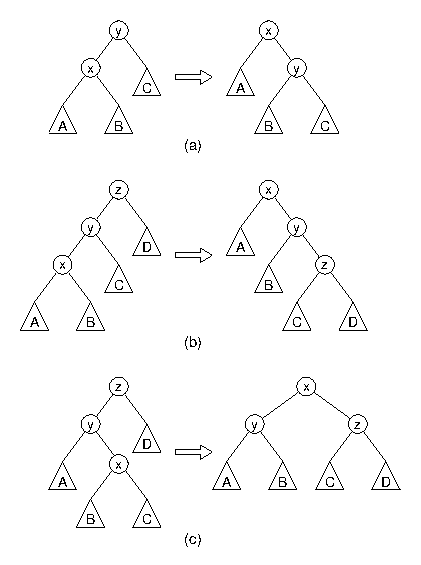
\includegraphics{images/fig1.eps}}
\caption{
ボトムアップ扁平化操作の1ステップ. % \cite{ST85}
$x$ がアクセスした節点.(a) zig: 1回の右回転($y$が根の場合
のみ),
(b) zig-zig: 枝$yz$と枝$xy$をこの順に右回転,(c) zig-zag: 枝$xy$
を左回転し,できた枝$xz$を右回転.}
\label{figure:splaying}
\end{figure}

扁平化はボトムアップな変形操作であるため,並列操作には適さない.
文献\Cite{ST85}はトップダウン扁平化も提案しているが,これは実装の
容易化が主な目的であり,木の根は操作終了の直前まで確定しない.


\subsection{並列操作に関する過去の研究}\label{subsection:related-parallel}

和田\cite{W90}は,並行論理型言語\cite{S89}の論理変数を用いた扁
平化アルゴリズムを提案している.これは,論理変数を利用して,
トップダウン扁平化をin-placeで行なうようにしたものと見なすこともできる
が,${\it update\/}$のように,対象となる節点が操作終了後の木に存在するこ
とがわかっている場合は,木の根のキーを操作の最初に確定させる点が大きな特徴で
ある.
%
% 数百節点の連続挿入操作の並列度は4〜8であるという実験結果が
% 報告されている\cite{W90}.
%
しかしこの技法は,
${\it delete\/}$のように,操作結果の木の根が事前にわから
ない場合には適用できない.


\subsection{トップダウン扁平化の問題点}

トップダウン扁平化による${\it update\/}$は,
\ref{subsection:related-parallel}節のように
根のキーを最初に確定させるよ
うにしても,並列処理の観点からは問題が残る.たとえば,節点
$x(<b)$ ($<$はキーによる順序関係)の${\it update\/}$によって起きる
図\ref{figure:topdown}の
zig-zig操作\cite{W90} を考える($L$と$R$は,木$C$をトップダウン扁平
化した結果の左(右)部分木で,${\it update\/}$完了時までに確定).

% \begin{adjustvboxheight}
\begin{figure}[tb]
  \centerline {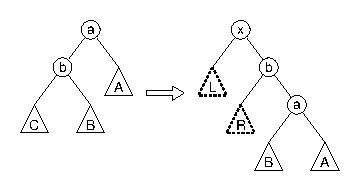
\includegraphics {images/fig2.eps}}
\caption{トップダウン扁平化による${\it update\/}$}
\label{figure:topdown}
\end{figure}
% \end{adjustvboxheight}

この${\it update\/}$の後,$y(<x)$, $z(>b)$へのアクセスがこの順に続くと
する.最初の$x$へのアクセス時に$x$が部分木$C$の左の方にあったためにzig-zig操作
が続く場合,$L$の
根が確
定するのは遅くなる.しかし$L$の根が確定するまでは,次の$y$へのアクセ
スがzig, zig-zig, zig-zagのどれをまず適用するか決められない.
%
% 長く待っても,目標の節点の上昇段数が多ければ問題はないのであるが,
% それが
%
そこで3番目の
$z$へのアクセスが,2番目の操作によって影響を受けることのない$b$の右部分
木に向かうにもかかわらず,長時間ブロックしてしまう.

削除操作はさらに問題である.一般に,二分木から節点$x$を削除するには,
$x$の左部
分木の最大の節点$y$を探してそれを$x$の場所に移すことが基本とな
る.しかし,扁平化の有無にかかわらず,$y$が見つかるまでは$x$の場所
にくる新たなキーは確定せず,後続の操作をブロックしてしまう.以下のよう
な解決法も考えられるが,いずれもうまく動作しない.

\begin{enumerate}
\item % {\bf 一時的なキー}
$y$が見つかるまで,$x$を一時的なキーとして利用すると,
$y\le z\le x$であるような節点$z$への操作を誤った方向へ導く.

\item % {\bf 双方向リスト}
各節点が直前と直後のキーをもつ節点へのポインタを保持することによって,
$x$の直前の要素$y$に${\rm O}(1)$時間でアクセスできるようにする
ことが考えられる.これらのポインタは木
の扁平化時に変更する必要がないという特徴がある.
%
しかしこの方法は逐次操作のときしかうまく動作しない.
%
% あるプロセスが節点
% $x$を削除しようとしたとする.そのプロセスは節点$y$に${\rm O}(1)$時間でア
% クセスできるものの,単にそれを削除して$x$のかわりに用いることはできない.
% (invisible pointer?)
%
なぜならこの削除操作の前の操作が$x$と$y$を結
ぶパスを下降中で,いずれ$y$に到達するかもしれないからである.
\end{enumerate}

したがって本論文では,高々${\rm O}(1)$個の節を施錠しつつ,厳密にトップダウ
ンに木を変形してゆくアルゴリズムを考えることとする.
